\section{A Refined View of Assurances} \label{sec:synthesis}
    From the review of Quadrants I. through IV. of the formal/informal, explicit/implicit plane (see figure \ref{fig:trust_assurance_intention}), we are able to find some insights with respect to assurances and can discuss them in a more comprehensive way. Using insights from the survey a refined version of figure \ref{fig:SimpleTrust_one_way} can be constructed. Figure \ref{fig:refined_assurances} incorporates all details from section \ref{sec:background} as well as adding some insights from the survey. The first insight is that both the AIA and the User must be able to perceive TRBs and the assurances respectively. Secondly, details about what make up assurances have been added to the `AIA Assurances' block. These changes will now be discussed in detail.

    \begin{figure}[htbp]
        \centering
        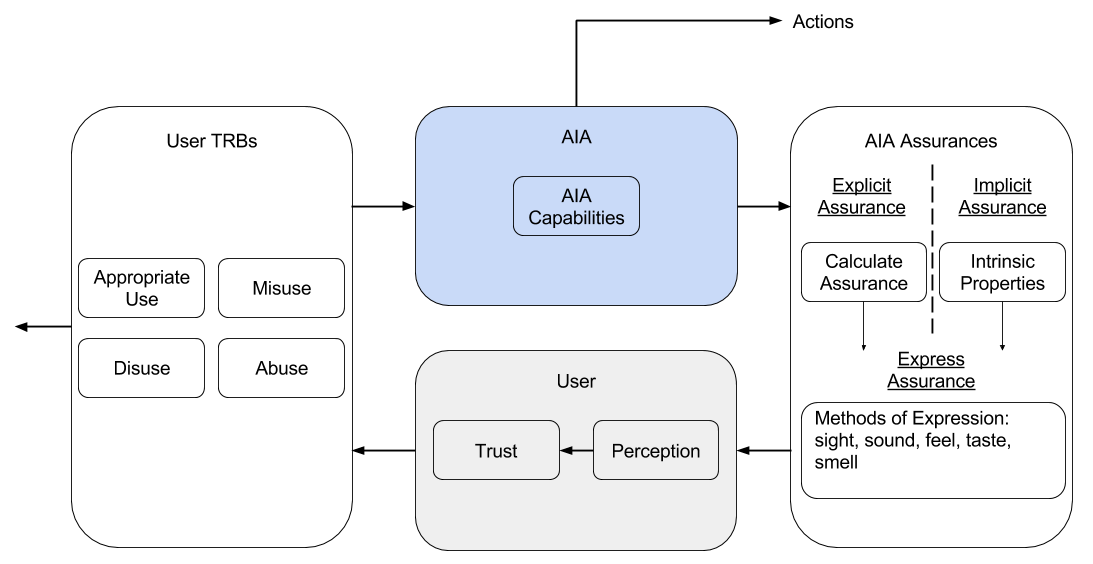
\includegraphics[width=0.9\textwidth]{Figures/RefinedTrust_one_way}
        \caption{Detailed extension of Figure \ref{fig:SimpleTrust_one_way}. The AIA, User , and User TRBs blocks are defined as discussed in section \ref{sec:background} (with the exception of the `Perception' blocks added to the AIA and User boxes). The AIA Assurances box has been filled using insights from the surveyed material.}
        \label{fig:refined_assurances}
    \end{figure}

\subsection{Calculating Assurances}
    % In order to give an assurance an AIA must first be able to create one, or more specifically the AIA must be able to calculate the information that needs to be conveyed. \cite{Kaniarasu2013-ho,Chen2014-dk} illustrate the kinds of assurances that can be created if they are designed from the beginning. However, most AIAs do not possess the ability to calculate assurances for their respective capabilities. AIAs must have the ability to be introspective (perform analysis on \emph{its own} functions, capabilities, and models, to compute assurances), as well as extrospective (perform analysis on the function, capabilities, and  models of \emph{external entities} to compute assurances). An AIA that possesses both together can be referred to as circumspective. Once circumspective analysis has occurred then the AIA must be able to express the assurances. This is a challenge that needs to be addressed directly, and the surveyed work (and other similar work) will help guide the development of those capabilities.

    In order for an AIA to give an assurance it must be able to calculate that assurance. It seems that there are a few high-level ideas that surround the calculation of assurances, these are: quantifying uncertainty, adding structure, and modifying the AIA objectives.

    \paragraph{Quantifying Uncertainty} Being able to quantify uncertainty in the AIA is a critical step in being able to express that uncertainty to a human user. The general idea is that a model or method needs to be incorporated in the AIA that will represent uncertainty in some way. A human user could use such information to inform their trust in the `situational normality', `competence', and `predictability' of the AIA. We claim that the work surveyed in the sections addressing \nameref{sec:performance_prediction}, \nameref{sec:model_checking}, \nameref{sec:safety}, \nameref{sec:active_learning}, and \nameref{sec:empirical_performance} can be used to this end. Generally these methods are statistical in nature, and directly account for uncertainty.

    One of the most popular methods was Gaussian Process models, which are able to represent uncertainty

    This is perhaps the most obvious of the methods to use when attempting to design assurances; In essence trying to provide another layer of information beyond a simple prediction, or recommendation. Generally the surveyed papers from quadrant \ref{sec:q2} found that including things like uncertainty increased the trustworthiness of the AIA in the user's eyes.

    \paragraph{Reducing Complexity} At the other end of the spectrum, many researchers attempted to remove complexity from the models and logic of the AIA to make the methods more interpretable to a human user. As with quantifying uncertainty, making an AIA more interpretable can also inform a user's trust in the `situational normality', `competence', and `predictability' of it. Many of the methods applicable were surveyed in the sections regarding \nameref{sec:model_interp}, \nameref{sec:explanation}, \nameref{sec:viz_dr}, \nameref{sec:human_involved},  and \nameref{sec:rep_learning}.

    Generally it is accepted in the surveyed literature that the models and algorithms of AIAs need to have less complexity in order to be better understood by human users. This reduction in complexity was addressed in several different ways. There was some investigation into how to make certain models more interpretable \edit{THIS NEEDS TO BE FINISHED}

    \paragraph{Modified Objectives} The above two approaches alone can largely use existing methods, however some researchers directly modified the methods and models in the AIA to be more meaningful to humans. This was reviewed to some extent in the sections on \nameref{sec:human_involved}, \nameref{sec:active_learning}, \nameref{sec:model_interp} (some researchers modified objectives to learn better models), \nameref{sec:rep_learning}, and \nameref{sec:safety}.

    When \citet{Freitas2006-qo} considered putting a human in the learning process, he essentially modified the objective function of the learning algorithm. In essence the objective function was now based on a large set of human preferences (and biases). This kind of approach is promising, in that it can be used to encode many human qualities that cannot be easily quantified, or even explained. These are trade-offs that can be undesirable in many situations as well. We sometimes use designed objective learning algorithms to avoid human biases. It is interesting that in using a human in the loop can offer more interpretability to a learning process, while at the same time making the learning process itself less procedural. In other words, using a human in the loop can make the result more understandable by a human, but the learning process will be rendered less understandable.

    \citet{Amodei2016-xi} discuss several different considerations related to AI safety, and spend quite a bit of time discussing the situation when AI objectives don't correspond, or align, with human objectives (this is something addressed in a specific situation by \cite{Hadfield-Menell2016-ws}, also \cite{Bostrom2012-uf}). One of the main insights is that the source of discord between what humans expect and what AIAs actually do is because of poorly designed objective functions that you might refer to as myopic, or focusing on a specific objective to the extent that a human can no longer relate to the objective of the AIA. This suggests to designers that significant time may be required to design objectives that align with human objectives, this alignment will automatically make the AIA more predictable, and competent in the user's eyes.

    \edit{old stuff\ldots, try and add in somewhere}
    reducing complexity can be seen in summarizing data for the user (i.e. calculating averages, summarizing distributions, dimensional reduction)
    modifying AIA objectives is a fundamental design change that takes human users into account. this is stuff from Dragan.

    To date several different promising methods have been used to calculate assurances in different applications. These include modifying the objective to consider a user's trust (i.e. legible motion \cite{Dragan2013-wd}, and safe learning), calculating intended actions, methods operating on POMDPs have also been developed in an attempt to quantify how they perform. Researchers from quadrant III and IV have developed many other promising approaches that involve predicting performance, making models more interpretable by simplifying them and/or adding structure, reducing the dimensionality, explaining the reasoning of decision making AIAs, checking models, guaranteeing performance through V\&V, learning safely, dealing with non-stationary training/test data, and learning better features. Many of these methods are ready (or nearly so) to be used in more formal human-AIA trust studies to verify their utility in this application.

    It is important to recognize the fact that AIAs may possess several different capabilities, and that each may be more or less trustworthy. This suggests that there must be several assurances created in order to assure the user with respect to each of the different capabilities. As discussed by \cite{Chen2014-dk} assurances from different capabilities may be more or less important depending on the situation (i.e. sometimes the user may need to understand why a decision was made, but not at other times).

\subsection{Expressing Assurances}
    The expression of assurances, calculated using methods from above, is a bit more complicated. This is because the expression can be directed at any of the human perceptions.

    An AIA must not only be able to calculate an assurance, but express it to the user as well. These expressions must be tailored to human strengths and weaknesses, some of which are mentioned in section \ref{sec:consider_human}. To state the point more bluntly, if an assurance is not expressed, or not perceived by the user, it is useless and has no effect. The expression of assurances to a human user is not a trivial topic and has been investigated mainly by those in quadrants I, and II by basic visualizations and natural language communication (some other promising approaches like high dimensional visualization were mentioned in quadrants III and IV). There is, however, a body of research (not surveyed here) that considers how to communicate information to humans (i.e. as probabilities, or fractions, by text, or by plotting, etcetera). It is probable that marketing, and cognitive science have much to contribute to this topic. This research is critical in designing how to efficiently express assurances in a way that they will be perceived correctly by the user with the least possible information loss.

    \paragraph{methods that have been used} plots, natural-language, projection of plans, summary statistics (outcome assessment, reliability), statistical distributions

    \paragraph{assurances that currently lack satisfactory expression} V\&V, methods that account for non-stationary distributions, feature representations there are opportunities here.

    \paragraph{certain capabilities lack appropriate methods} i.e. POMDPs don't have a method of quantifying solver quality (i.e. competence), are there assurances for POMDP `situational normality' or `predictability'?

    \edit{this has some cross-over with the previous section} Part of expression is user preference, the other part is cognitive limitations. Do plots work better? Or does speech? Use a male voice or female? Use slang when expressing via natural language?

\subsection{Perception of Assurances}
    A user will always have some kind of TRB towards an AIA (if only to choose to ignore the AIA). In the absence of explicit assurances the human will instead use implicit assurances to inform their TRBs. However, the human user will not have knowledge regarding which assurances are implicit or explicit. In other words the user won't necessarily be able to distinguish which assurances were designed and which weren't. To the user all assurances are the same, that is to say that any property or behavior of an AIA that affects trust is an assurance, and it doesn't matter whether the assurance was designed or not (is explicit or implicit). As illustrated in Figure \ref{fig:refined_assurances}, perception of the assurance is the first step in which the human user is involved. This highlights the idea that human perception (both sensory and cognitive) needs to be taken into account when designing assurances.

    An important consideration when designing assurances is whether a human can perceive the assurances being given. If so, to what extent is the information from the assurance transfered (i.e. how much information was lost in the communication)? A few examples include: an AIA giving an auditory assurance in a noisy room and the user not hearing it (such as an alert bell in a factory where the workers use ear-plugs), or an AIA attempting to display an assurance to a user that has obstructed vision. Much of the research to date involves assurances that are not robust to loss in transfer, due to the use of methods that use a single medium of expression. Because of this, exploring ways in which assurances can be robustly communicated is a clear opportunity for those trying to design assurances. This is akin to a human speaking with their voice, making facial expressions, and gestures with their hands as well; all of those methods of communication together help transfer information with less loss.

    In this survey we saw several different mediums used to convey an assurance. Some used sight such as in \cite{Chadalavada2015-wx} where the robot gave visual feedback to a user, or in \cite{Muir1996-gt} where performance data were visible on a computer screen. Others used sight as well when communicating via natural language (i.e. \cite{Wang2016-id}) -- it is also a simple matter to convert natural language output from visual to auditory with existing technology. Generally, any human sense could be used as a medium, besides sight, and sound this includes touch, smell, and taste. None of the last three have formally been investigated in human-AIA trust relationships to our knowledge. Although it should be said that haptic feedback (where the user receives mechanical feedback through the robot controls) is frequently used as a part of a more immersive user interface in robotics. Taste and smell have an obvious application in the assurances of a cooking robot.

    \edit{I want to add something here about assurances over time, i.e. teaching a person}

    \paragraph{Implicit and Explicit Assurances:} \edit{look at this again} It is worth considering, in more detail, what implications this has on the designer. The foremost consideration is that an analysis of the interaction between the human and user need to be made in order to identify the critical assurances for a given scenario. For example, in the road network problem, an analysis might find that the most critical assurances are about the competence of the UGV's planner. In this case the designer must take time to design a planning-competence assurance.

    One difficulty arises form this approach, which is that there doesn't seem to be a way to determine what passive assurances might drown out active assurances. Following from the example above, the designer may have built an excellent planning-competence assurance, but failed to consider the effect of how the UGV appears -- it may be old, have loose panels, and rust holes. \edit{it is common to overlook certain passive assurances because you assume they will be `normal', for example build a UGV and it will be pretty much like any other vehicle. --- a possible way to think about this would be to go through each AIA capability and consider the different perceptions that a user might have, and then ask whether those perceptions would be `typical', if not, and active assurance should be designed}

    \paragraph{human-like assurance:} What perceptions are beneficial to a certain task? Constrasting \cite{Dragan2013-wd} and \cite{Wu2016-ei} shows that sometimes the same technique can have different effects when used in different situations. In \cite{Dragan2013-wd} the AIA is made more trustworthy by making the robot motions more human-like, whereas in \cite{Wu2016-ei} making the AIA more human-like resulted in a decrease of trustworthiness. In this case the difference came from the type of task, in the first case the robot was physically working in proximity to a human, in the other case the user was playing a competitive game against the AIA.

    \edit{What does it even mean to make something more "human-like"? In the cases above this meant to move in a more human way, and to act more human, by delays and others. There has been some work that also studies the effects of the presence of humanoid robots. \textbf{I think part of what matters is considering the purpose of the AIA, is it supposed to be more human? or is it supposed to be better/different than a human?}}

    \paragraph{Assurance Efficiency:} Perhaps less obvious is a situation in which the user has to supplement an incomplete assurance. \edit{this might also be seen as a under-powered, or ineffective explicit assurance} As a simple example, in \cite{Muir1994-ow} a simple flow-rate is provided to the user, they then supposedly create a mental model of the reliability -- based on repeated observations over time of the AIA to inform their TRBs. Creating this mental model takes time, and the model is prone to cognitive biases (discussed a bit more below).

    A highly efficient assurance would have precise information communicated in a way that is easy for the user to perceive. Inefficient. \edit{talk more about this}
    
    \paragraph{User Cognition:} A second more nuanced point is whether the user can process the information received. This is perhaps most easily illustrated by considering a non-expert user who cannot understand highly technical assurances regarding the AIA. However, less trivial manifestations may be troubling. This point was not directly addressed in the survey papers, but evidence of its existence were seen. For example in quadrant I \cite{Riley1996-qm}, and \cite{Freedy2007-sg} both observed evidence of framing effects (the tendency of a user to become too trusting once they are in the mode of trusting). This suggests the existence of other kinds of typical cognitive behaviors such as recency effects (having biased trust based on recent experiences). With these cognitive affects we see that the human brain inherently has limitations to being able to process assurances correctly. These limitations must be considered when designing assurances.

    \edit{discuss how recency effects might come in to play}

    \edit{discuss perhaps some other kind of cognitive bias}

\subsection{Measuring the effects of Assurances}

    There are two different situations when it would be desirable to measure the effects of assurances. The first is when the designer wants to understand the effectiveness, the second would be when the AIA itself needs to measure whether assurances are effective or not. To our knowledge there has not been any work regarding the second situation where an AIA would measure response to assurances and then adapt behaviors appropriately (at least not in the trust cycle setting), however this is arguably the ultimate goal so that AIAs can themselves modify assurances to meet different needs. What does this mean practically? It seems that any method that is made for the designer to measure the effects of assurances could also be deployed into an AIA. The surveyed literature gives some insights into how that has been done to date.
   
    When it comes time to measure the effect of assurances on a human's trust there are two main approaches. The first is self-reported changes based on questionnaires, the second involves measuring changes of user's TRBs. The questionnaire approach was used extensively in many of the papers surveyed, questions like `how trustworthy do you feel the system is?', or `to what extent do you find the system to be interpretable?'. These kinds of questions can be useful in verifying whether the assurances are having the expected effect. It is not unreasonable to imagine that an AIA might be equipped with a method by which it can ask the user questions about their trust, process those responses, and modify assurances appropriately.
    
    However, evidence is presented in \cite{Dzindolet2003-ts} that illustrates that sometimes changes is self-reported trust do not result in changes in TRBs. From the AIAs perspective this means that --- unless the object of the assurances is to make the person's level of self-reported trust change --- the assurances are not providing any benefit. As previously discussed, the goal of assurances is to elicit appropriate TRBs from the human user. From this perspective, measuring changes in TRBs is the more objective approach to measure the effect of assurances.

    Generally researchers in the field have measured, in some way, how frequently the AIA was able to run in autonomous mode, before being turned off. This metric seems very reasonable, and seems to be a promising approach with some extensions. Perhaps a better defined metric would be the likelihood of appropriate use of a certain capability by the user. For example in the UGV road-network example there isn't really an option to `turn off' the UGV. Instead the remote operator can make decisions such as accepting a plan designed by the UGV. In this situation the effect of assurances might be measured by how likely the operator is to accept a generated plan instead of overriding it (recall that the goal may not be to have the generated plan accepted 100\% of the time, rather that it be accepted with respect to how appropriate it is in a given situation).

    Self-reports are likely the most useful when trying to understand the true effects of an assurance. Does a certain assurance, assumed to affect `situational normality', actually do that? There is space for quite a lot of research in this realm. Does displaying a specific plot actually convey  information about `predictability'? This information can be used to inform the selection of the methods of assurance.

    In practical application (such as in the UGV road-network problem), the user, and the human-AIA team, care more about whether TRBs are appropriate or not. It doesn't help if an assurance helps the user feel that the AIA is more competent, if the user doesn't treat the AIA any differently than before the assurance. This assumes that it is possible for appropriate TRBs be measured in the first place. For example, if appropriate behavior is for the user to verify a sensor reading, can the AIA perceive that? In that situation perhaps the easiest approach would be to ask the user, but what if the user lied? Is there a way to verify the TRB is actually appropriate? This is something that has gained notoriety with autonomous cars, where the car can drive itself, but the user still needs to sit in the driver's seat and be attentive just in case the vehicle cannot perform correctly. We claim that it is as important to design methods of perceiving appropriate (and inappropriate) TRBs as it is to design assurances. 


\subsection{The Imprecise Nature of Assurances}
    Due to the nature of trust (and humans in general), a single assurance might be targeted at influencing the competence dimension of trust, but it may also have effects on other dimensions. As an example an assurance that targets predictability may also have an affect on the probability of depending.

    Besides being difficult to separate effects on a single user, individual users are different as well. Thus no assurance will have an identical effect when given to two separate users. This makes it difficult to have precise effects on user trust behaviors.

    One might attempt to mitigate this uncertainty by using expressions that are more precise than others, such as displaying a probability distribution rather than on a maximum likelihood. This gets into some considerations about how the presentation of information affects the ability of a human to understand.
%
% \subsection{Classes of Assurances}
    % Given the considerations discussed above, we can make some attempt at classifying assurances.
    % \subsubsection{Explicit and Implicit Assurances}
\citet{Sheridan1984-kx} briefly alluded to the existence of explicit and implicit assurances when they discussed the nature of how humans behave when working with automated systems. They suggested that the operator's perception of the automated system can be effected by `performance' and its `reports on its own performance'. 


\begin{description}
    \item [Explicit:] Assurances that are purposefully given to affect the trust of a user.
    \begin{itemize}
        \item Legible motion \cite{Dragan2013-wd}, which is motion calculated with the intent of being more understandable by a human
        \item $R^2$ value, gives some indication of how well the regression accounts for the variance of the data
    \end{itemize}
    \item [Implicit:] All other assurances that aren't explicit.
    \begin{itemize}
        \item Reliability in completing a task. Generally, the object of success is not to affect the user's trust (although this is a nice side-effect).
        \item The way an autonomous vehicle appears. For example something that looks neat will have a different effect on trust, than an AIA with wires dragging on the ground. 
    \end{itemize}
\end{description}



    % \subsubsection{Source-Target Classification}
    It is convenient to refer to assurances by way of their source and target. Intuitively, there may be a set of different algorithms that are useful for making assurances that convey information about planning to the competence dimension of the user's trust. It is easier to refer to these assurances in terms of their source and target. So, for this example that class of algorithms would be the `planning-competence' class.
    
    Not only is this useful shorthand for communicating about the purpose of the algorithms, but it is useful in classifying the range of assurance algorithms that exist. There may also be a class of algorithms that span multiple source-target capabilities. For example there may be a kind of algorithm that can give a `learning-competence' assurance, as well as a `planning-competence' assurance.

    This is especially true since many of the AIA capabilities can overlap. Also, the effects of assurances cannot be guaranteed to affect only one trust dimension.

    Figure \ref{fig:Assurance_classes} shows the hierarchy of proposed assurance classes. The categories mirror those of the trust model proposed by \citet{McKnight2001-fa}, but with the emphasis on what an AIA has the ability to most readily influence (and consequently where most research is found). The boxes with the beveled corner identify and define the different classes of assurances. All classes are included here for completeness and generality. Although, while it is hypothetically possible for an AIA to influence a persons general `Trusting stance' given enough time\footnote{One might imagine an AIA that specifically speaks to the human about the benefits or drawbacks about trusting even though there might not be evidence to do so, similar to the role a counselor might play}, the gray boxes are not considered further in this survey, as practically no direct research exists in the realm of human-AIA relationships.

    \textbf{ugggg, this gets a little complicated, but it's not supposed to be}.

    % \subsection{Component and Composite Assurances}
Assurances can be either component or composite. This was seen a little through the survey. The definitions are as follows:

\begin{description}
    \item [Component:] An assurance that originates from a single AIA capability source, and targets a single trust dimension target.
    \item [Composite:] The combination of more than one component assurance into a single assurance. 
\end{description}

\begin{figure}[!htbp]
    \centering
    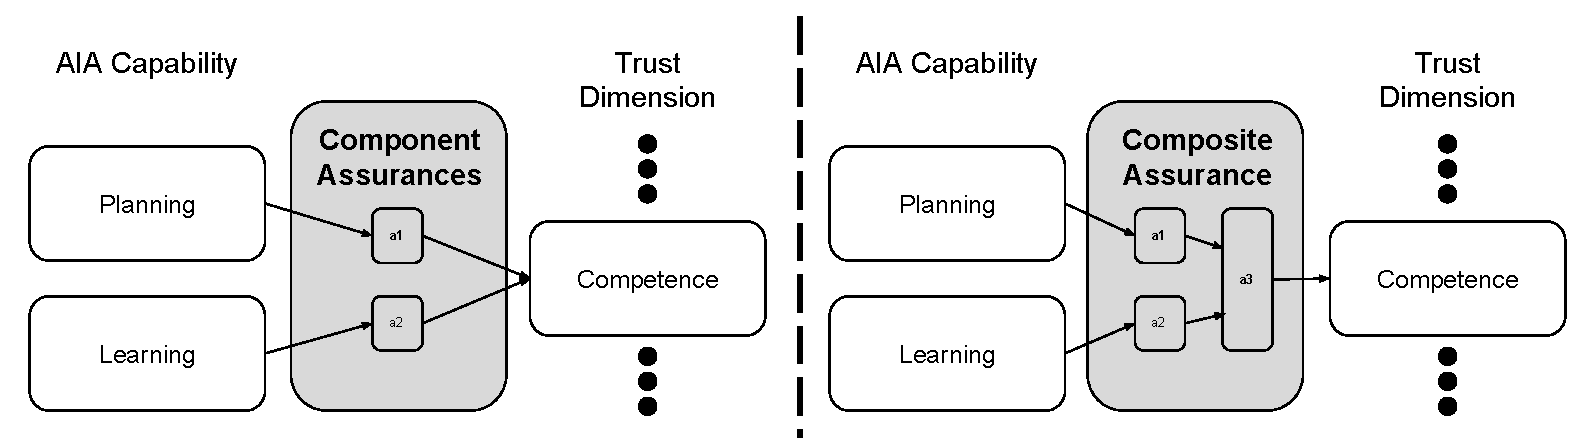
\includegraphics[width=0.9\textwidth]{Figures/Assurance_component_composite.pdf}
    \caption{Figure illustrating the difference between component and composite assurances. The existence of multiple assurances does not imply a composite assurances, rather the combination of multiple component assurances into a single assurance constitutes a composite assurance.}
    \label{fig:assurance_mapping}
\end{figure}

Figure \ref{fig:assurance_mapping} illustrates the concepts of component and composite assurances.

\paragraph{Component Assurances:} Component assurances are perhaps the most well researched in the existing literature. This is likely because several verified component assurances are the predecessors to composite ones. A component assurance might include displaying the confidence of a classification prediction, or visualizing a model as discussed in section \ref{sec:q2}.

\paragraph{Composite Assurances:} Composite assurances are assurances that are built of several components. A notable example is the work by \citet{Aitken2016-cv} who propose a measurement called `self-confidence', applicable to Partially Observable Markov Decision Processes (POMDPs). This metric combines five component assurances into a single composite assurance that is meant to distill the information into a value that a novice operator could understand easily. This paper was discussed in more detail in \ref{sec:q2}. 

    % \emph{Tutoring vs Telling:}
Most assurances investigated to date are `telling', in that they do not consider the experience or other traits of different users. The ability to adapt to different users, and to tutor them to appropriate trust will become more critical as time passes due to the diversity of users bases for advanced AIAs and time that users will interact with them. A tutoring assurance would be a planned, dynamic, sequence of assurances that would change in time to adapt to the user's needs. This might include modification of assurances to help a user avoid boredom, or to use the system differently in varying circumstances. It isn't surprising that, to our knowledge, no research has been done with respect to tutoring a user in a trust relationship. This is a complex problem to address that would involve understanding how different users learn, and what an appropriate strategy would be to teach them to have appropriate TRBs. However, a rich resource (not investigated in this paper) would be the work on tutoring systems \citet{Wenger2014-ld} and algorithmic teaching \citet{Balbach2009-jw}.

